\typeout{IJCAI-16 Instructions for Authors}

\documentclass{article}
% The file ijcai16.sty is the style file for IJCAI-16 (same as ijcai07.sty).
\usepackage{ijcai16}

% Use the postscript times font!
\usepackage{times}

% the following package is optional:
%\usepackage{latexsym} 

% author added packages
\usepackage{xspace}

\newcommand{\ispy}{\textit{I, Spy}\xspace}

\title{Grounded Attribute Learning with Multi-Modal Perception}
%\title{Learning Multi-Modal Grounded Linguistic Semantics by Playing ``I Spy''}
\author{Paper XXX}
%\author{name \\ 
%affiliation  \\
%email}

\begin{document}

\maketitle

\begin{abstract}
	% The abstract should be no more than 200 words long
	We build models of object attributes that use visual, haptic, auditory, and proprioceptive perceptual data acquired through robot exploratory behaviors using supervision from human-robot interaction.
\end{abstract}

\section{Introduction}
\label{sec:introduction}
Robots need to be able to connect language to their environment in order to discuss real world objects with humans.
Mapping from referring expressions such as ``the blue cup'' to their object referents in the world is part of the \textit{symbol grounding problem}~\cite{harnad:phys90}.
Symbol grounding involves connecting internal representations of information in a machine to real world data from its sensory perception.
\textit{Grounded language learning} bridges these symbols with natural language.

Early work on grounded language learning enabled a machine to map between adjectives and nouns such as ``red'' and ``block'' to objects in a scene through vision-based classifiers~\cite{roy:evocomm01}.
We refer to adjectives and nouns that describe properties of objects as language \textit{predicates}.
Most work has focused on grounding language predicates through visual information. However, other sensory modalities such as haptic and auditory are also useful in allowing robots to discriminate between objects~\cite{sinapov:icra14}.
This paper explores grounding language predicates by considering visual, haptic, auditory, and proprioceptive senses. 

A home or office robot can explore objects in an unsupervised way to gather perceptual data, but needs human supervision to connect this data to language.
Learning grounded semantics through natural human-robot dialog allows a system to acquire the relevant knowledge without the need for laborious labeling of numerous objects for every potential lexical descriptor.
A few other groups have explored learning from interactive linguistic games such as \ispy and ``20 Questions'' \cite{parde:ijcai15,vogel:aaai10}; however, these studies have been restricted to simple objects and only employed vision (see Section \ref{sec:relatedwork}).

\begin{figure}
\centering
\begin{tabular}{c}
	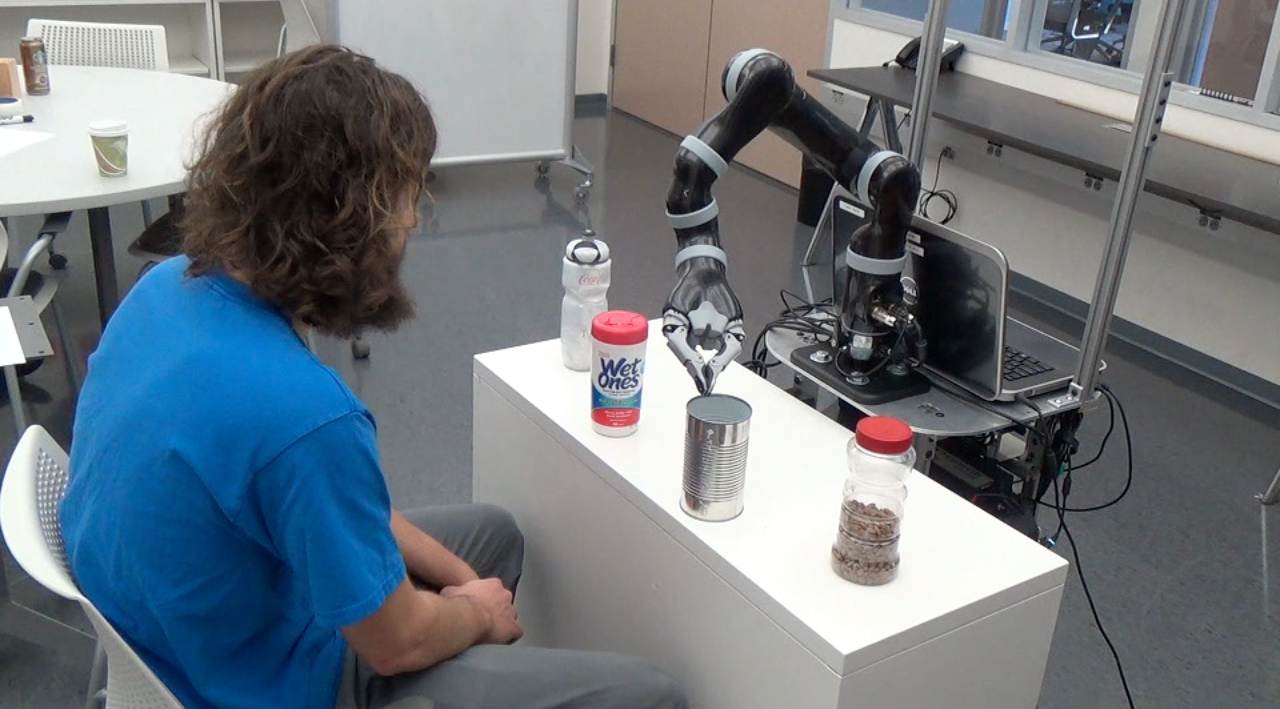
\includegraphics[width=0.3\textwidth]{figures/silver_round_and_empty.png} \\
	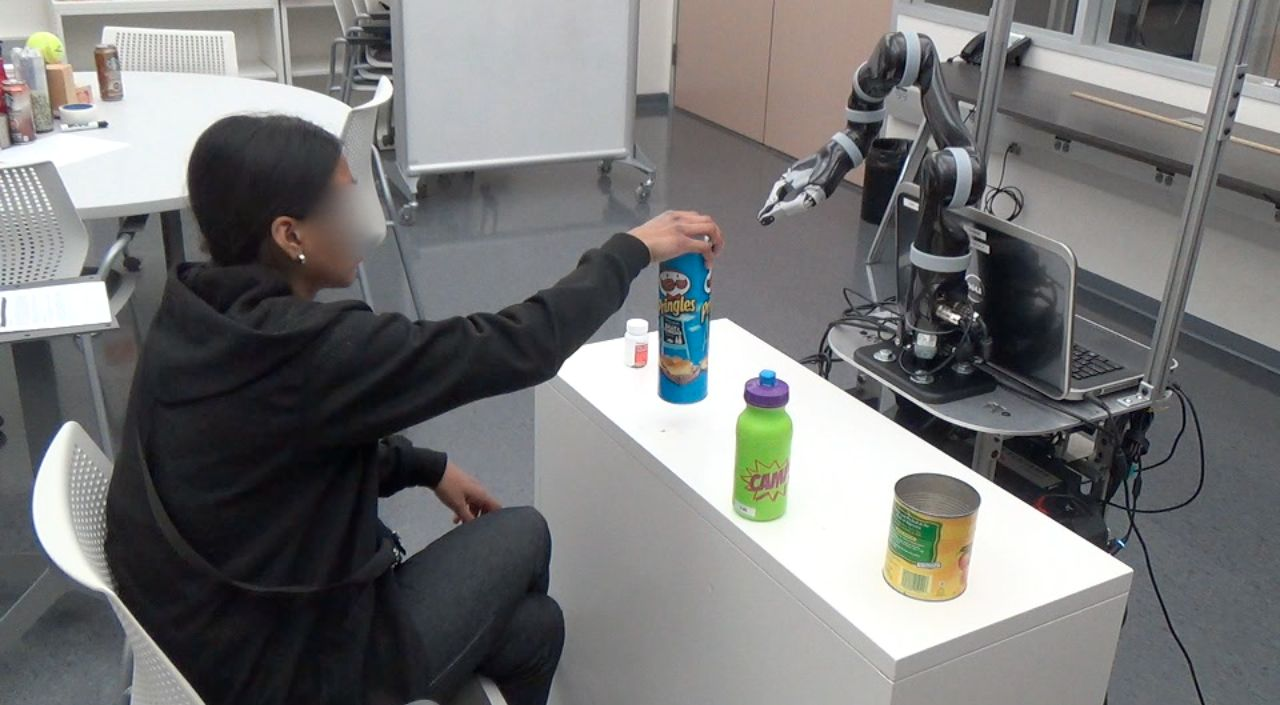
\includegraphics[width=0.3\textwidth]{figures/light_tall_tub.jpg} \\
\end{tabular}
\caption{\textbf{Top}: the robot guesses an object described by a human subject as ``silver, round, and empty.'' \textbf{Bottom}: a human subject guesses an object described by the robot as ``light,'' ``tall,'' and ``tub.''}
\label{fig:ispy}
\end{figure}

We use a variation on the children's game \ispy, as a learning framework for gathering human language labels for objects to learn multi-modal grounded lexical semantics.
Figure~\ref{fig:ispy} shows the players (humans and the robot) guessing an object the other has described.
Our experimental results test generalization to new objects not seen during training and illustrate both that the system learns accurate word meanings and that modalities beyond vision improve its performance.

To our knowledge, this is the first robotic system to perform natural language grounding using multi-modal sensory perception through feedback with human users.

\section{Related Work}
\label{sec:relatedwork}
% relation to grounded language learning tasks
Researchers have made substantial progress on grounding language for robots, enabling tasks like object recognition and route following from verbal descriptions. 
Early work used vision together with speech descriptions of objects for this learning~\cite{roy:cogsci02}.

In the past few years, much of this work has focused on combining language with visual information. 
For grounding referring expressions in an environment, many learn perceptual classifiers for words like `red', `square', and `left' given some pairing of human descriptions and labeled scenes~\cite{liu:acl14,malinowski:nips14,mohan:acs13,sun:icra13,dindo:iros10,vogel:aaai10}. 
Some works additionally incorporate language models into the learning phase~\cite{spranger:ijcai15,krishnamurthy:acl13,perera:aaai13,matuszek:icml12}. 
Our method uses simple language understanding and constructs new attribute classifiers for new, unseen words used by a human playing \ispy. 
Unlike any previous methods, our classifiers take advantage of more than just visual data from objects.

Including a human in the learning loop provides a more realistic learning scenario for applications such as household robotics. 
Past work has used human speech plus gestures describing sets of objects on a table as supervision to learn attribute classifiers~\cite{matuszek:aaai14,kollar:rss13}. 
Recent work introduced the \ispy game as a framework for supervision~\cite{parde:ijcai15} for grounded language learning. 
Outside of robotics, there has been some work on combining language with other sensory modalities than vision, such as audio~\cite{kiela:emnlp15}. 
Our work differs from these in that we use experience gathered from more than vision to build object attribute classifiers. 
In our instantiation of the \ispy task, the robot and the human both take a turn describing objects, where in previous work~\shortcite{parde:ijcai15} only the human played this role. 
To our knowledge, ours is the first work to integrate visual, haptic, auditory, and proprioceptive information for language grounding by an embodied robot.

% relation to multi-modal perception (i.e. jivko's work)
% TODO: jivko

\section{Task Definition}
\label{sec:taskdefinition}
In our \ispy task, the human and robot take turns describing objects from among four on a tabletop [[Figure picture??]].
There are two rounds of turns in each game. In each round, the human subject starts by describing and object of her choice.

Subjects were asked to describe objects through their attributes, as opposed to singling them out as instances.
As an example, we suggested subjects describe an object as ``black rectangle'' as opposed to ``whiteboard eraser.''
Additionally, subjects were told they could handle the objects physically before offering a description, but were not asked to use non-visual predicates.
Once subjects offered a description, the robot guessed the objects it most thought the subject was talking about in order (see section~\ref{ssec:gll}) until one was confirmed correct.

In the second half of each round, the robot picked an object and then described it with up to three predicates (see section~\ref{ssec:gll}).
The subject was again able to pick up and physically handle objects before guessing.
The robot confirmed or denied each subject guess  until the right object was chosen.

The \ispy game admits two clear metrics.
The \textit{robot guess} metric is the number of turns the robot took to guess what object the subject was describing.
The \textit{human guess} metric is the number of turns the human took to guess what object the robot was describing.
Using these metrics, we compare the performance of two \ispy playing systems as described in section ~\ref{sec:experiment}.

\section{Object Dataset}
\label{sec:dataset}
\begin{figure}
\centering
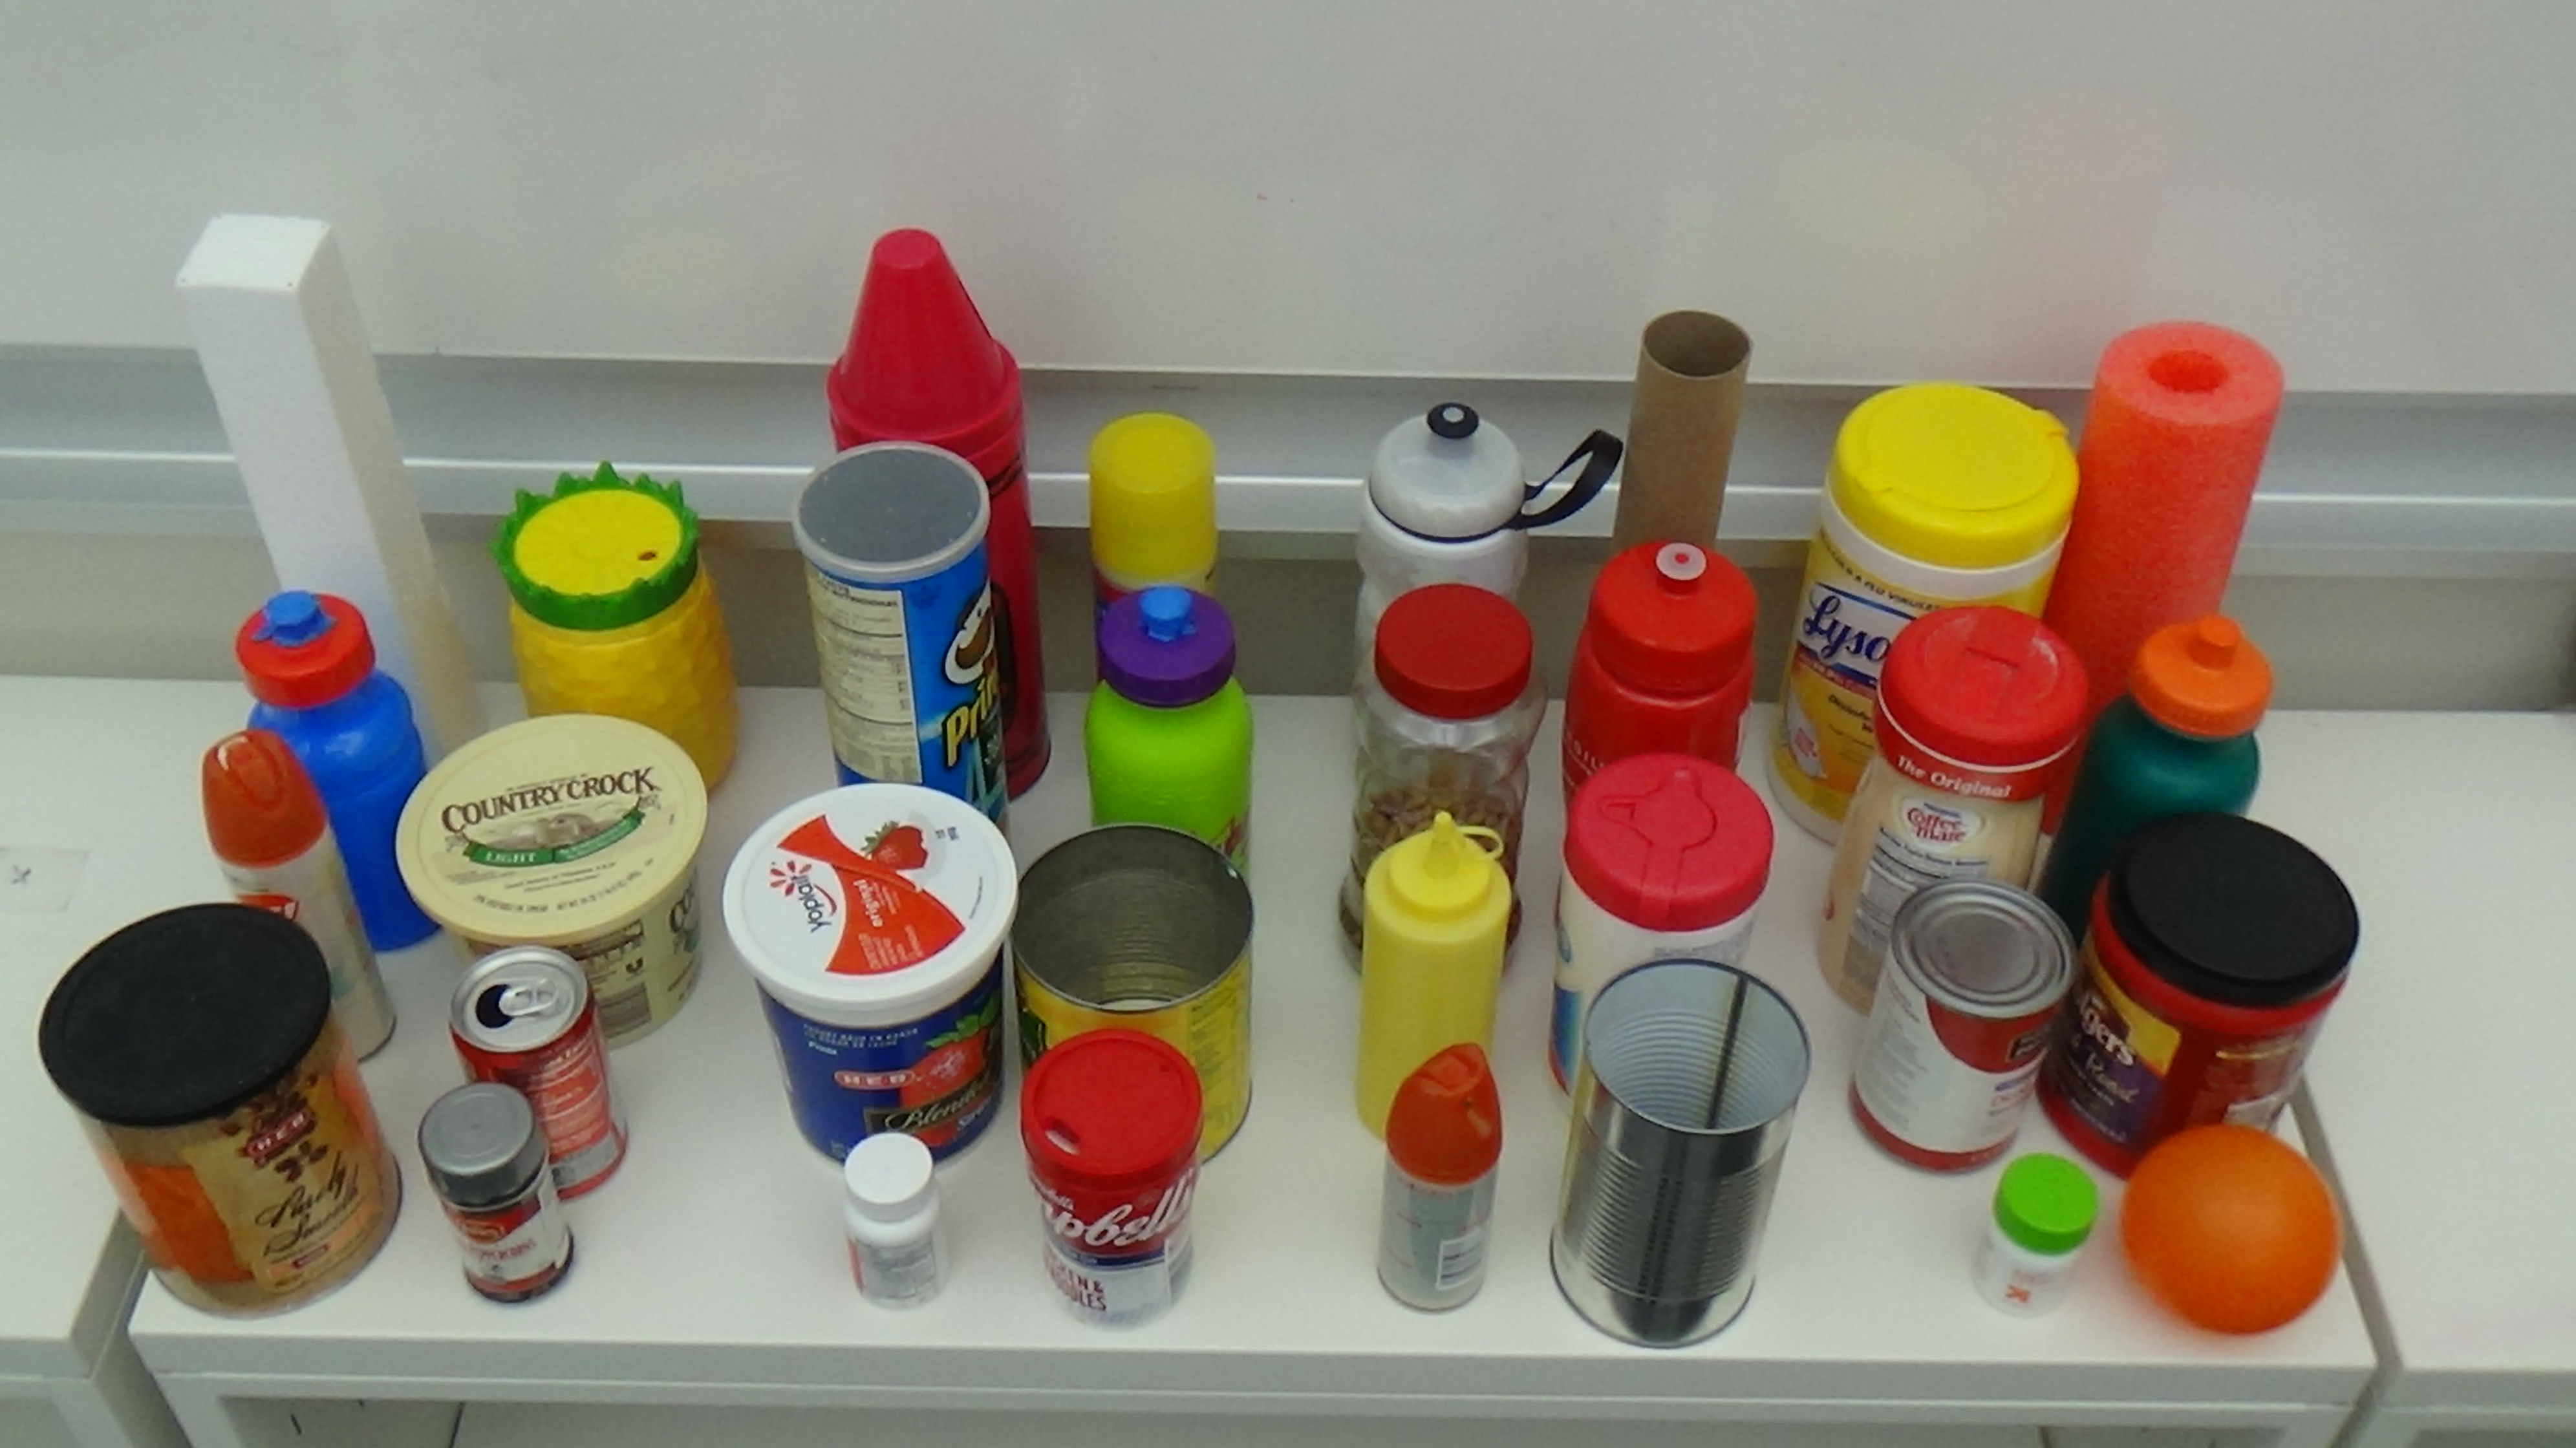
\includegraphics[width=0.3\textwidth]{figures/objects.jpg}
\caption{Objects used in the \ispy game divided into the four folds discussed in Section~\ref{ssec:methodology}, from fold 0 on the left to fold 3 on the right.}
\label{fig:objects}
\end{figure}

The robot used in this study was a Kinova MICO arm mounted on top of a custom-built mobile base, which remained stationary during our experiment.
The robot's sensors included joint effort sensors in each of the robot arm's motors, a microphone mounted on the mobile base, and the Xtion ASUS Pro RGBD camera.
The set of objects used in this experiment consisted of 32 common household items including cups, bottles, cans, and other containers, shown in Figure~\ref{fig:objects}.
Some of the objects contained liquids or other contents (e.g., coffee beans) while others were empty.
Contemporary work gives a more detailed description of this object dataset~\cite{sinapov:ijcai16}, but we briefly describe the exploration and modalities below.

\subsection{Exploratory Behaviors and Sensory Modalities}
\label{ssec:contexts}

\begin{center}
\begin{figure}[t]
\setlength{\unitlength}{1in}
 \centerline{
\begin{picture}(3.5,2.5)
\put(0.0,1.4){\psfig{file=figures/behaviors/grasp1.eps,width=1.1in}}
\put(0.4,1.275){grasp}
\put(1.2,1.4){\psfig{file=figures/behaviors/lift1_arrow.eps,width=1.1in}}
\put(1.7,1.275){lift}
\put(2.4,1.4){\psfig{file=figures/behaviors/lower1_arrow.eps,width=1.1in}}
\put(2.8,1.275){lower}
\put(0.0,0.075){\psfig{file=figures/behaviors/drop1.eps,width=1.1in}}
\put(0.45,-0.05){drop}
\put(1.2,0.075){\psfig{file=figures/behaviors/press1_arrow.eps,width=1.1in}}
\put(1.6,-0.05){press}
\put(2.4,0.075){\psfig{file=figures/behaviors/push2_arrow.eps,width=1.1in}}
\put(2.8,-0.05){push}
\end{picture}
}
\caption{The behaviors the robot used to explore the objects.
The arrows indicate the direction of motion of the end-effector for each behavior.
In addition, the {\it hold} behavior (not shown) was performed after the {\it lift} behavior by simply holding the object in place for half a second.}
\label{fig:behaviors}
\end{figure}
\end{center}
\vspace {-5mm}

Prior to the experiment, the robot explored the objects using the methodology described by Sinapov et al.~\shortcite{sinapov:ras14}, and the dimensionality of the raw auditory, haptic, and proprioceptive data were reduced comparably (final dimensionality given in Table~\ref{tab:feature_space_of_contexts}).
In our case, the robot used 7 distinct actions: {\it grasp}, {\it lift}, {\it hold}, {\it lower}, {\it drop}, {\it push}, and {\it press}, shown in Figure~\ref{fig:behaviors}.
During the execution of each action, the robot recorded the sensory perceptions from {\it haptic} (i.e., joint efforts) and {\it auditory} sensory modalities.
During the {\it grasp} action, the robot recorded {\it proprioceptive} (i.e., joint angular positions) sensory information from its fingers.
The joint efforts and joint positions were recorded for all 6 joints at 15 Hz.
The auditory sensory modality was represented as the Discrete Fourier Transform computed using 65 frequency bins.

In addition to the 7 interactive behaviors, the robot also performed the {\it look} action prior to grasping the object which produced three different kinds of sensory modalities: 1) an RGB color histogram of the object using 8 bins per channel; 2) Fast point feature histogram ({\it fpfh}) shape features~\cite{rusu:icra09} as implemented in the Point Cloud Library~\cite{aldoma:ram12}; and 3) deep visual features from the 16-layer VGG network~\cite{simonyan:corr14}.
The first two types of features were computed using the segmented point cloud of the object while the deep features were computed using the 2D image of the object. 

\begin{table}
\centering
\begin{tabular}[h]{|l|c|c|c|}
	\hline
	\bf Behavior & \multicolumn{3}{c|}{\bf Modality} \\ \hline \hline
	& \bf color & \bf fpfh & \bf vgg \\ \hline
	\bf look & 64 & 308 & 4096 \\ \hline \hline
	& \bf audio & \bf haptics & \bf proprioception \\ \hline
	\bf grasp & 100 & 60 & 20 \\ \hline
	\bf drop, hold, & & & \\
	\bf lift, lower, & 100 & 60 & \\
	\bf press, push & & & \\ \hline
\end{tabular}
\caption{The number of features extracted from each \textit{context}, or combination of robot behavior and perceptual modality.}
\label{tab:feature_space_of_contexts}
\end{table}

Thus, each of the robot's 8 actions produced two to three different kinds of sensory signals.
Each viable combination of an action and a sensory modality is a unique sensorimotor context.
In our experiment, the set of contexts $\mathcal{C}$ was of size  $2 \times 3 + 6 \times 2 = 18$.
The robot performed its full sequence of exploratory actions on each object 5 different times (for the {\it look} behavior, the object was rotated to a new angle each time). Given a context $c \in \mathcal{C}$ and an object $i \in \mathcal{O}$, let the set $\mathcal{X}_i^c$ contain all five feature vectors observed with object $i$ in context $c$.
	% overview that data was gathered using arm behaviors
	% TODO: jivko

\section{Implementation}
\label{sec:implementation}
	To play \ispy, we first gathered sensory data from the set of objects through robot manipulation behaviors (described in Section~\ref{sec:dataset}).
When playing a game, the robot was given unique identifying numbers for each object on the table and could look up relevant feature vectors when performing grounding.

During the course of the game, the robot used its RGBD camera to detect the locations of the objects and subsequently detect whenever a human reached out and touched an object in response to the robot's turn.
The robot could also reach out and point to an object when guessing.
We implemented robot behaviors in the Robot Operating System\footnote{\texttt{http://www.ros.org/}} and performed text-to-speech using the Festival Speech Synthesis System.\footnote{\texttt{http://www.cstr.ed.ac.uk/projects/festival/}}

	\subsection{Multi-Modal Perception}
	\label{ssec:mmp}

		% object dataset and arm behaviors data collection

	\subsection{Grounded Language Learning}
	\label{ssec:gll}
	Language predicates and positive/negative labels for those predicates were gathered through human-robot dialog during the \ispy game.
The human subject and robot were seated at opposite ends of a small table.
A set of 4 objects were placed on the table for both to see.
We denote the objects on the table during a given game as set $\mathcal{O}_T$.

\paragraph{Human Turn.} On the subject's turn, the robot asked him or her to pick an object and describe it in one phrase.
We used a standard stopword list to strip out non-content words from the subject's description.
The remaining words were treated as a set of language predicates, $\mathcal{H}_p$.
The robot assigned scores $S$ to each object $i\in \mathcal{O}_T$ on the table.
\begin{equation}
	S(i) = \sum_{p\in \mathcal{H}_p}{G_p(i)}
\end{equation}
The robot guessed objects in descending order by score (ties broken randomly) by pointing at them and asking whether it was correct.
When the correct object was found, it was added as a positive training example for all classifiers  $p\in \mathcal{H}_p$ for use in future training.

\paragraph{Robot Turn.} On the robot's turn, an object was chosen at random from those on the table.
To describe the object, the robot scored the set of known predicates learned from previous play.
Following Gricean principles~\cite{grice:bkchapter75}, the robot attempted to describe the object with predicates that applied to it but did not ambiguously refer to other objects on the table.
We use a predicate score $R$ that rewards describing the chosen object $i^*$ and penalizes describing the other objects on the table.
\begin{equation}
	R(p) = |O_T|D_p(i^*) - \sum_{j\in{\mathcal{O}_T}\setminus\{i^*\}}{D_p(j)}
\end{equation}
Note that this scoring equation also rewards predicates for describing $i^*$ while clearly {\it not} describing the other objects on the table (\textit{e.g.}  $D_p(j)<0$).
The robot choose up to three highest scoring predicates $\hat{P}$ to describe object $i^*$ to the subject, using fewer if $S<0$ for remaining predicates.
Once ready to guess, the subject touched objects until the robot confirmed that they had guessed the right one ($i^*$).

The robot then pointed to $i^*$ and engaged the user in a brief follow-up dialog in order to gather both positive and negative labels for $i^*$.
In addition to predicates $\hat{P}$ used to describe the object, the robot selected two additional predicates $\bar{P}$.
$\bar{P}$ were selected randomly with $p\in P$ having a chance of inclusion proportional to $1-|G_p(i^*)|$, such that classifiers with low confidence in whether or not $p$ applied to $i^*$ were more likely to be selected.
The robot then asked the subject whether they would describe the object $i^*$ using each $p\in\hat{P}\cup\bar{P}$.
The subject's responses to these questions provided additional positive/negative labels to the classifiers of these predicates for use in future training.


\section{Experiment}
\label{sec:experiment}

	% overview

	\subsection{Methodology}
	\label{ssec:methodology}

		% folds to allow incremental learning and results; way folds were formed

		% description of handout and instruction video

		% description of setup wrt operator being a transcription service

	\subsection{Results}
	\label{ssec:results}

		% average robot turns to guess human pick over folds; average human turns to guess robot pick over folds; statistical comparison to true random (0.25), maybe fold-fold tests too
		% if enough users return, can do paired tests of fold0-fold3 for example

\section{Conclusion}
\label{sec:conclusion}

% \section*{Acknowledgments}

%% The file named.bst is a bibliography style file for BibTeX 0.99c
\newpage
\bibliographystyle{named}
\bibliography{/u/ml/bib/lunar,/u/jesse/local}

\end{document}
